% ----------------------------------------------------------
% Arquivo contendo a introdução do trabalho sobre algoritmo genético
%
% ----------------------------------------------------------
\chapter{Introdução}
% ----------------------------------------------------------

\section{Algoritmos evolucionários}

Os algoritmos evolucionários são um subconjunto da computação evolutiva, sendo essa um conjunto de algoritmos para busca de soluções ótimas globais. A computação evolutiva é baseada na evolução das espécies definida na biologia, e assim os algoritmos evolucionários se baseiam em processos encontrados na natureza de seleção, reprodução e mutação das espécies, com o propósito de otimizar a solução para um problema definido.

Um problema de otimização é definido como maximizar, ou minimizar, $f(x)$ sujeito a \(g_i(x) \leq 0\,i = \{1,\ldots, m\}\), e \(h_j(x) = 0, j=\{1,\ldots,n\}\) com \(x \in \Omega \). A solução maximiza, ou minimiza, o escalar \(f(x)\) onde \(x\) é um vetor com dimensão \(n\), \(x=\{x_1,x_2,\ldots,x_n\}\) do espaço de soluções \(\Omega\). \cite{Coello2007} 

Dessa forma o problema de otimização tem os seguintes componentes:
\begin{itemize}
	\item Função objetivo \(f(x)\): função de avaliação que deve se minimizada ou maximizada;
	\item As restrições \(g_i(x)\) e \(h_j(x)\): definem limites para as soluções que são permitidas;
	\item Espaço de soluções \(\Omega\) :
		Conjunto com todas as possíveis soluções para o problema; 
\end{itemize}

De forma mais simplificada podemos escrever o problema de otimização como, sendo \(\Omega\) o espaço de soluções e a função \[ g: \Omega \to \mathbbm{R}\] e a solução o vetor \(x \in \Omega\) tal que \[ \arg \min \limits_{x \in \Omega} g(x)\] que pode facilmente ser convertido para um problema de maximização usando \(-g(x)\)

Para atingir esse objetivo os algoritmos evolutivos trabalham com uma população de indivíduos que indicaremos como soluções candidatas para o problema. Baseado na avaliação de cada individuo com relação ao seu ambiente, em nosso contexto a função de avaliação, e usando operadores definidos para seleção e evolução, a população vai sendo modificada até que se atinja um resultado satisfatório para o problema. Assim como no processo de evolução das espécies definidos por Darwin, que introduziu o conceito de seleção natural  através da sobrevivência do mais apto, os indivíduos da população que tem melhores avaliações, ou seja, que melhor se adaptam ao ambiente, possuem mais probabilidade de sobrevivência e assim se reproduzirem. 

Existem vários métodos para se otimizar um problema conforme pode ser visto na \autoref{fig:classificacao_metodos_busca}. Existem os métodos enumerativos, que se tornam impraticáveis quando o \(\Omega\) é muito grande, pois o algoritmo deveria testar todas as soluções possíveis. Os algoritmos determinísticos são os mais eficientes em determinadas condições, como por exemplo o comportamento de \(f(x)\). Se a função objetivo possui múltiplos máximos (ou mínimos) alguns algoritmos determinísticos, como o \textit{hill-climbing} por exemplo, podem ficar 'presos' em soluções locais e não encontrar a solução global. A última categoria, onde se encontram também os algoritmos evolucionários, são os estocásticos (ou randômicos). Possuem a vantagem de não ficar presos em soluções locais, porém nem sempre obterão a melhor solução.

\begin{figure}
	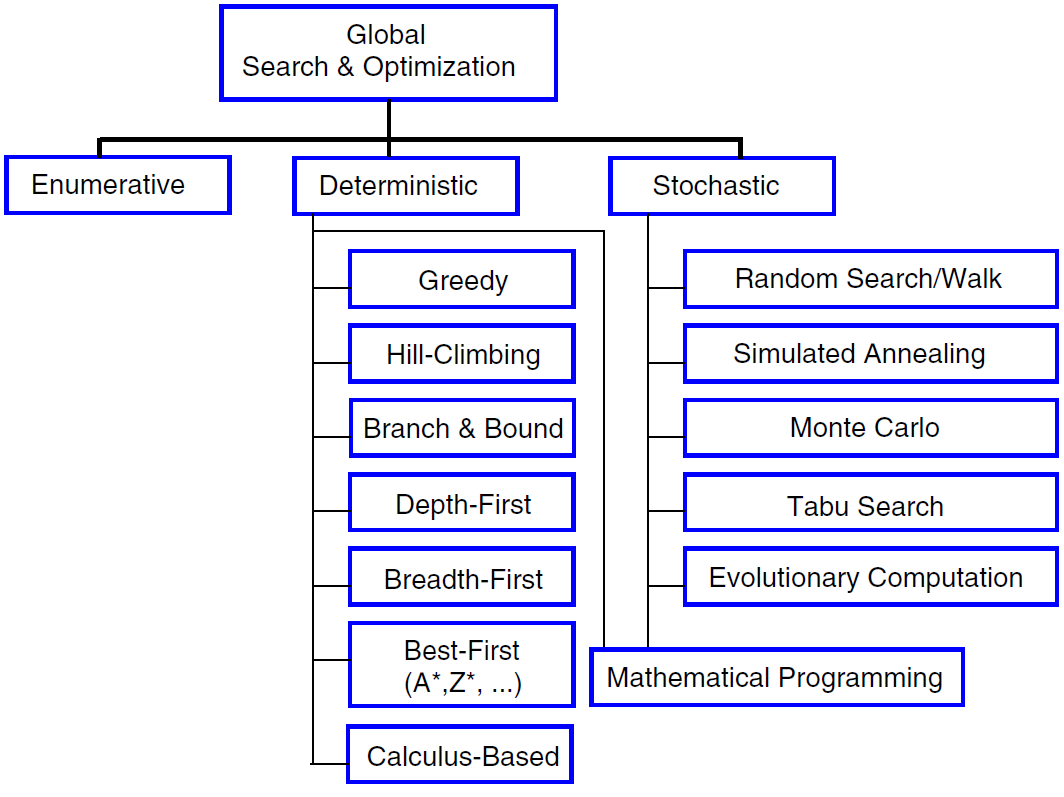
\includegraphics[width=\linewidth]{imagens/classificacao_metodos_busca.png}
	\caption{Técnicas de otimização global - \cite{Coello2007}}
	\label{fig:classificacao_metodos_busca}
\end{figure}

Dentre a categoria dos métodos estocásticos existem os que são completamente aleatórios, como a busca randômica (ou passeio aleatório), e os que são de alguma forma guiado como o método de Monte Carlo por exemplo. O algoritmo evolucionário se encaixa nessa ultima definição, onde existem componentes aleatórios atuando na seleção e reprodução dos indivíduos mas de forma guiada pelos resultados da função de avaliação.

De acordo com \citeauthor{Linden2008}, os AE são \textbf{heurísticas}\footnote{Heurísticas são algoritmos polinomiais que usualmente tendem a encontrar soluções ótimas ou próximas delas, mas sem garantias} que não asseguram obter o melhor resultado possível, e além disso o resultado pode diferir entre as execuções do algoritmo.

Para \citeauthor{Sivanandam2007}, um algoritmo evolucionário são processos estocásticos e iterativos que operam em um conjunto de indivíduos (população). Cada individuo representa uma possível solução para o problema de otimização ou busca, sendo que os parâmetros estão de alguma forma codificados nesses indivíduos. A população inicial é gerada aleatoriamente e são avaliados usando alguma função, que determina o quão bem o indivíduo responde ao problema. Esse valor determina a direção de busca do algoritmo. 

\section{Biologia}
A ideia por trás dos algoritmos evolucionários e por consequência do algoritmo genético, é a teoria de evolução das espécies na natureza de \textbf{Darwin}, onde a sobrevivência de cada indivíduo é determinada por como ele se adapta ao seu meio. Assim aqueles que conseguiam vantagens sobre os demais por ter uma maior sobrevivência se reproduziam mais, e assim, passavam para as próximas gerações essas características que os diferenciavam. Darwin chamou de seleção natural esse mecanismo da sobrevivência dos mais aptos.

Contudo Darwin não sabia explicar como essa informação era passada dos ancestrais para os descendente, onde então entram as descobertas de \textbf{Mendel}, que através dos conceitos de genética determinava como características eram compartilhadas entre pais e filhos. 

A unidade básica de informação é o gene, que é um bloco de sequências de DNA e o conjunto de genes formam o cromossomo. Cada gene tem um \textit{locus}, que define a região dentro do cromossomo onde está localizado, e possui um conjunto de valores possíveis chamados de alelos. Os genes controlam as características do indivíduo, sendo que a expressão dessas no individuo é denominada de fenótipo. Assim um conjunto específicos de genes define o genótipo do indivíduo que está associado a um fenótipo, que apresenta as características codificadas no genótipo e que podem ser modificadas pelo ambiente. 

Organismos com cromossomos combinados em pares são chamados de diplóides em contraste com os que não possuem pares, chamados de haplóides. Na natureza a maioria dos seres mais complexos que se reproduzem sexualmente são normalmente diplóides e possuem um ou mais pares de cromossomos sendo que sua quantidade e tamanho dependem de cada ser vivo.

Durante a reprodução ocorre a transmissão da informação que pode ser de dois tipos: assexuada e sexuada. Na reprodução assexuada, o organismo replica a si mesmo, presente mais em seres simples, não representa tanta diversidade pois como não existe combinação de material genético entre dois seres, ocorre apenas a retransmissão de material genético, somente sujeito a alterações por mutação na cópia.

Na reprodução sexuada de seres diplóides, há presença de dois indivíduos que compartilham seu material genético para formar um novo organismo. No inicio da reprodução, existe a cópia do material genético e recombinação, também chamado de \textit{crossover}(\autoref{fig:crossover_example}). Esse processo é feito com é feito com os cromossomos se cruzando, por isso o termo \textit{crossover},  um sobre o outro em um ou mais pontos havendo assim a troca nas sequências de genes. Após feita a recombinação, o material genético é divido em gametas que então são combinados com os gametas do outro pai para formar novamente um cromossomo diplódie completo, gerando assim os novos indivíduos. Para organismos haplóides é feita apenas a combinação das sequencias de cada pai.

\begin{figure}
	\begin{center}
	\includegraphics[width=0.5\textwidth]{imagens/cross_over.png}
	\caption{Exemplo de reprodução com crossover - \cite{Klug2011}}
	\label{fig:crossover_example}
	\end{center}
\end{figure}


Dentro da etapa de replicação do DNA podem ocorrer erros ou alterações influenciadas por fatores externos, gerando assim as mutações. Isso pode ser positivo, negativo ou não influenciar o resultado final, mas é um outro mecanismo que pode determinar a evolução das espécies.

Os genes definem as características dos indivíduos, mas também existe interação entre os genes, chamada de epistasia(\textit{epistasis}), podendo um par de genes mascarar ou modificar a característica final de outro par de genes. \cite{Klug2011}. Isso é importante do ponto de vista do algoritmo genético pois nem sempre a melhor avaliação estará associada a um único parâmetro, podendo estar associado a uma combinação de parâmetros.

Mendel ainda definiu o conceito de dominância-recessividade em organismos diplóides, assumindo que cada característica é controlada por pares de genes, sendo recebidos um de cada pai. Assim um dos alelos do gene é dominante sobre o outro apresentando a característica final no individuo, e outro alelo será considerado recessivo.

Combinando indivíduos que melhor se adaptaram as condições de sobrevivência, provavelmente deve gerar novos indivíduos que tenha características ainda melhores que seus antecessores. O outro caso pode acontecer também e o novo indivíduo ter piores condições de viver, e assim o processo de seleção natural levará esse espécime a extinção favorecendo outros que se sobressaíram na próxima geração.

A evolução então é um processo adaptativo onde através de mutações e recombinação entre os indivíduos, vão surgindo novas gerações que devem apresentar cada vez mais seres que se adaptam cada vez melhor ao ambiente.

\section{Surgimento do algoritmo genético}

Os algoritmos evolucionários vem sendo estudados a um longo tempo, desde da década de 40 que os cientistas se inspiram na natureza para criar os primeiros passos para a inteligência artificial, passando pela década de 50 onde começam os estudos sobre sistemas adaptativos para gerar soluções candidatas para problemas de difícil solução. Na década de 60 Rechenberg desenvolveu as estratégias evolucionárias (\textit{evolutionary strategies}) usando cromossomos compostos de números reais para estudos com aerofólios. Também apareceu a programação evolucionária, usando estruturas de pequenas máquinas de estados para resolver determinadas tarefas, que evolui para programação genética onde pequenos programas passam a ser as soluções candidatas. Existiram outros trabalhos sobre algoritmos evolucionários, programação evolucionária e algoritmos genéticos nas áreas de otimização e aprendizado de máquina, porém foram os trabalhos de Holland nas décadas de 60 e 70 que consolidou os algoritmos genéticos. \cite{Mitchell1996, Linden2008}

Alguns autores como \citeauthor{Mitchell1996}, \citeauthor{LeeJacobson2015}, \citeauthor{Kwong2001} entre outros citam Holland como criador do algoritmo genético(\textit{Genethic Algorithm} ou GA) em 1975 no livro \textit{"Adaptation in Natural and Artificial Systems"}. Nele Holland formaliza uma estrutura para sistemas adaptativos, e encaixa o GA como uma abstração para a evolução biológica.

O objetivo de Holland não era fazer algo especifico mas sim analisar os sistemas adaptativos e criar uma solução computacional que simulasse os processos encontrados nos sistemas de adaptação natural. Para isso cria uma abstração da evolução na biologia usando uma estrutural formal teórica que poderia atender diversos sistemas evolutivos e não somente o GA. Na formulação do GA por ele, os cromossomos seria representações binárias e utilizou os operadores de crossover, inversão e mutação inspirados na genética. O fato de ter usado cromossomos binários serviu de influencia para vários outros estudos que se seguiram, mas será exposto no \autoref{chap:GA} que existem outras formas de representar os cromossomos que dependem exclusivamente do problema a ser estudado.

O algoritmo genético geral proposto por Holland se baseia em uma população de cromossomos com alelos '0' e '1' e com os operadores de crossover, mutação e inversão. As evoluções seguiam os seguintes passos: 
\begin{enumerate}
	\item \label{en:loop} Seleção de um cromossomo na população de forma estocástica baseada nas avaliações de todos os cromossomos
	\item \label{en:gene} Aplicações dos operadores genéticos sobre uma cópia do individuo selecionado em \ref{en:loop}.
	\item Seleção de outro cromossomo de forma aleatória com probabilidade igual para todos a ser substituído pelo novo cromossomo gerado em \ref{en:gene}
	\item Avaliar o novo cromossomo
	\item Retonar ao \ref{en:loop}
\end{enumerate}

Essa é uma descrição bem resumida sobre o algoritmo e serve de base para as derivações. Por exemplo no caso do uso de um operador de crossover no \autoref{en:gene}, há a necessidade de seleção de outro cromossomo para formar um par e assim gerar uma nova estrutura.

Avaliando o algoritmo, temos alguns itens básicos que estarão presentes. A codificação do cromossomo para representar os parâmetros das soluções para os problemas. Uma população de cromossomos que serão avaliados simultaneamente durante as iterações do processo. A função de avaliação, que baseada nos parâmetros de cada estrutura irá fornecer uma forma de comparar os diversos elementos presentes na população. Os operadores genéticos que serão usados, sendo que podem ser combinados de diversas formas. 

De acordo com \citeauthor{Mitchell1996} existem 3 operadores para o algoritmo mais simples:
\begin{description}
	\item[Seleção] seleciona cromossomos favorecendo os que tem melhor função de avaliação
	\item[Crossover] também chamado de recombinação, combina dois cromossomos na geração de um novo
	\item[Mutação] Altera de forma aleatória alguns alelos dos cromossomos por exemplo em uma codificação binária seria alterar um dos bits do parâmetro.
\end{description}

No \autoref{chap:GA} será explorado com mais detalhes cada um dos operadores. Holland também descreve um operador de inversão, que apesar de garantir uma melhor diversidade genética impõe uma carga computacional grande para os ganhos efetivos, e nos trabalhos mais recentes se tornou um operador quase nunca usado.

Outro teoria que Holland formula sobre os GAs é em relação ao processo de paralelismo intrínseco, sobre a forma do algoritmo trabalhar com esquemas em vez de testar indivíduos específicos da população. \citeauthor{Goldberg1989} aborda esse tema com a hipótese dos blocos de construção (\textit{Building block hypothesis}).

\section {Teorema da inexistência do almoço grátis}
Existe um compromisso entre a eficiência de um algoritmo e sua robustez, isso é, ele pode ser muito eficiente para determinados problemas mas serem ineficientes em outros. Isso implica que não existe um algoritmo que seja eficiente para todos os problemas, e então é razoável supor que algoritmo genético tenha melhor eficiência em determinadas situações. Essa falta de um algoritmo universal é comparado por \citeauthor{Spall2003} a busca de uma agulha no palheiro sem nenhum dado sobre sua posição. Para essa situação a busca aleatória seria um dos melhores métodos de busca e em média nenhum outro seria mais eficiente.

Essa falta de um algoritmo universal para solução dos problemas de otimização parte do teorema da inexistência do almoço grátis (NFL - \textit{No-Free-Lunch Theorem}) proposto por Wolpert. O NFL ainda afirma que todos os algoritmos de busca tem em média o mesmo desempenho\cite{Linden2008}. O que de fato deve ser chamado a atenção é que apesar do apelo do algoritmo comparado com a evolução da espécies, é que se houver um método específico para determinado problema, definitivamente ele será mais eficiente que o GA.

Na \autoref{fig:NFL} \citeauthor{Goldberg1989} mostra que no espectro de problemas de busca e otimização, um método especializado em determinado problema sempre terá a maior eficiência e que os métodos aleatórios e enumerativos apesar de serem considerados menos eficientes podem ter desempenho melhor que o método específico em um espectro mais amplo. O método robusto representa um algoritmo idealizado para solução dos problemas em todas as variedades de problemas. Seria interessante ter um algoritmo robusto, mesmo abandonando o pico de eficiência pois assim atenderia uma variedade de problemas. Como tal algoritmo não é conhecido o que pode ser feito é usar métodos híbridos combinando mais de uma técnica.

\begin{figure}
	\begin{center}
		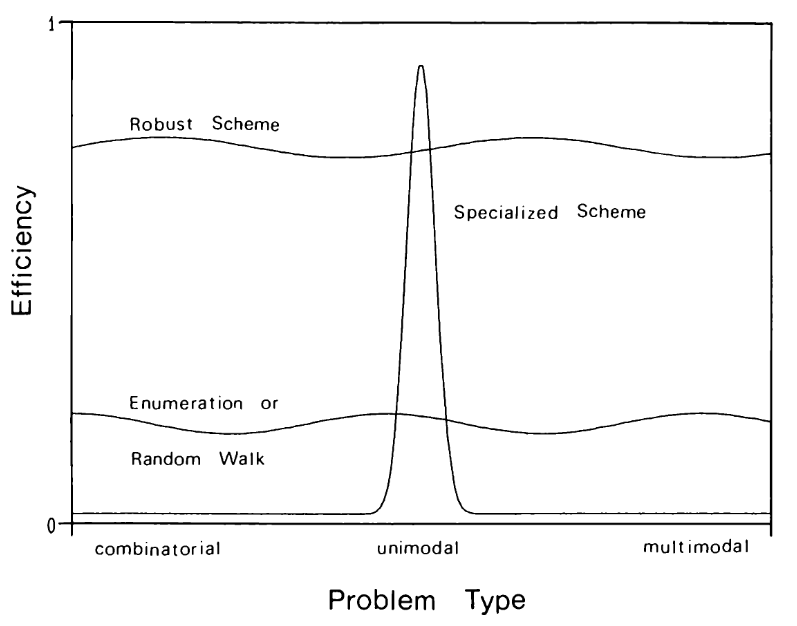
\includegraphics[width=0.5\textwidth]{imagens/David_NFL_Theorem.png}
		\caption{Exemplo para NFL - \cite{Goldberg1989}}
		\label{fig:NFL}
	\end{center}
\end{figure}
